\documentclass[12pt, a4paper]{article}
\usepackage{tikz}
\usepackage{makra}
\usepackage{hyperref}
\usepackage{indentfirst}
\usepackage{makeidx}
\usepackage{graphicx}
\usepackage{caption}
\usepackage{subcaption}
\makeindex
\renewcommand{\thesection}{\arabic{section}.}
\renewcommand{\thesubsection}{\arabic{section}.\arabic{subsection}.}
\renewcommand{\thesubsubsection}{\arabic{section}.\arabic{subsection}.\arabic{subsubsection}.}
\usepackage{qtimes}
\newcommand{\przepis}{\textbf{USTAWA
z dnia 29 lipca 2005 r.}


o ofercie publicznej i warunkach wprowadzenia instrumentów finansowych do zorganizowanego systemu obrotu oraz o spółkach publicznych''}
\def\thesection{\arabic{section}}
\author{W.~Łojkowski}
\title{Crowfunding}
\date{14.12.2014}

\linespread{1.2}

\begin{document}
\maketitle

\tableofcontents


\newpage
\section{Crowdfunding - co to jest?}
\label{sec:wstęp}


	Crowdfunding\index{crowdfunding} jest formą finansowania różnego rodzaju projektów przez społeczność, która otrzymuje w zamian różnego rodzaju benefity (np. w postaci wcześniejszego dostępu do produktu końcowego). Przedsięwzięcie jest w takim przypadku finansowane poprzez dużą liczbę drobnych, jednorazowych wpłat dokonywanych przez osoby zainteresowane projektem. Crowfunding zaczął się niezwykle dynamicznie rozwijać dopiero na przestrzeni ostatnich kilku lat, dzięki łatwemu dostępowi do projektów przez odpowiednie serwisy internetowe. Za kolebkę crowdfundingu\index{crowdfunding} uznaje się Stany Zjednoczone Ameryki. W roku 1997 amerykańscy fani brytyjskiej grupy rockowej Marillion w wyniku przeprowadzonej w internecie kampanii zebrali 60 tysięcy dolarów na sfinansowanie trasy koncertowej tegoż zespołu po Stanach Zjednoczonych. W późniejszym okresie zespół Marillion wykorzystał tą metodę finansowania przy tworzeniu albumów „Anoraknophobia”, „Marbles” i „Happiness Is the Road”.
	
	\begin{quote}
"Sukces należy do tych, którzy wierzą w potęgę swoich pomysłów" - Michael Irwin. Jedno z najważniejszych haseł promujących crowdfunding\index{crowdfunding}.
\end{quote}

\begin{figure}[h]
	\centering
		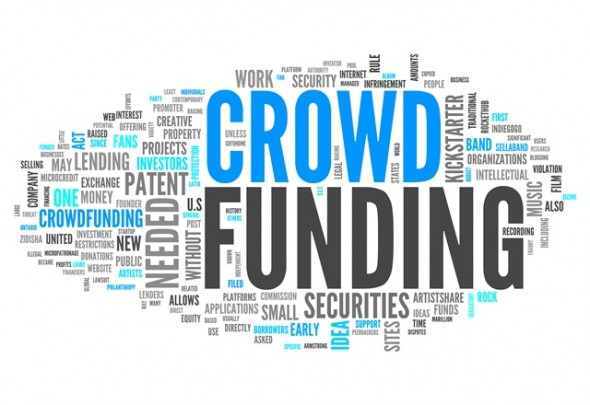
\includegraphics[width=0.50\textwidth]{crow.jpg}
	\caption{}
	\label{fig:images}
\end{figure}
\newpage

\section{Platformy crowdfundingowe\index{crowdfunding} na świecie}
\label{sec:platf}

 Pierwszy serwis, który umożliwiał wspieranie twórców przez społeczność ukazał się w 2000 roku i był dostępny pod adresem: ArtistShare.net\index{Artist Share}, na łamach którego ogłaszali się głównie muzycy i artyści. Następny duży serwis pojawił się dopiero w 2008 roku o nazwie Indiegogo\index{Indiegogo}. Obecnie największym serwisem i najmłodszym z wcześniej wymienionych jest Kickstarter\index{Kickstarter} (powstały w 2012 roku). Wszystkie wspomniane serwisy powstały w Stanach Zjednoczonych.

Najważniejsze cechy tego typu serwisów:
\begin{enumerate}
\item Można składać projekty z różnych dziedzin, takich jak: Sztuka, Komiksy, Społeczność, Taniec, Design, Wydarzenia, Moda, Jedzenie, Wideo/film, Gry, Książki/Publikacje, Dziennikarstwo, Muzyka, Fotografia, Technologia, Teatr, Edukacja, Podróże, Sport.
\item Nie obsługują projektów charytatywnych.
\item Nie obsługują finansowania biznesów, tylko projekty.
\item Nie obsługują projektów, w realizacji których projektodawca nie uczestniczy.
\item Wszystkie projekty muszą oferować nagrody, za ich wspieranie.
\item Projektodawcy ustalają dolny limit kwoty, którą chcą pozyskać, jeżeli nie uda im się zebrać tej kwoty w czasie trwania akcji, nie dostają oni nic. Jeżeli kwota przewyższy dolną granicę, twórcy dostają całą zebraną kwotę odejmując około 10\$ na rzecz serwisu.
\end{enumerate}

%Loga serwisów
\begin{figure}[ht!]
    \centering
    \begin{subfigure}{.4\linewidth}
        
\includegraphics[scale=0.3]{kic}
    \end{subfigure}
    \hskip2em
    \begin{subfigure}{.4\linewidth}
        
\includegraphics[scale=0.3]{ind}
    \end{subfigure}
    \begin{subfigure}{.4\linewidth}
        
\includegraphics[scale=0.3]{pob}
    \end{subfigure}
    \caption{Several subfigures}
\end{figure}

\newpage

\subsection{Jak to działa?}
\label{sec:jakd}

Zasada działania Kickstartera\index{Kickstarter} jest bardzo prosta. Osoba z pomysłem zakłada projekt na stronie. Ustala minimalny budżet jaki jest potrzebny do ruszenia produkcji i ustala nagrody za wsparcie projektu odpowiednią kwotą. Następnie, osoba której projekt się spodoba zgłasza chęć jego wsparcia podając dane swojej karty płatniczej. Całą obsługa płatności zajmuje się Amazon Payments\index{Amazon Payments}. Podając dane karty i wybierając nagrodę środki nie są ściągane z naszego konta, a tylko blokowane. Oznacza to nie mniej nie więcej, że jeśli projekt nie osiągnie zakładanego minimum środki zostaną nam zwrócone. Możemy też w każdej chwili nasze finansowanie edytować. Kickstarter\index{Kickstarter} za wszystko pobiera drobną prowizję. Oczywiście, jeśli projekt zakończy się sukcesem. Niestety na dzień dzisiejszy projekty można zgłaszać tylko ze Stanów Zjednoczonych, oraz Wielkiej Brytanii. Początkowo były to tylko Stany Zjednoczone. Wielka Brytania pojawiła się dosyć niedawno (stąd w niektórych projektach pojawiły się funty). Jednak osoba wspierająca może być już z każdego miejsca na świecie. Tłumaczeniem takiego obrotu spraw było początkowo korzystanie właśnie z Amazon Payments, jednak teraz jak dodano Wielką Brytanie można mieć nadzieję, że coś się zmienia.

Opłaty pobierane przez określony serwis możemy obliczyć, używając poniższych wzorów (gdzie x to zebrana kwota):


\[
 \left\{
 \begin{matrix}
  x\times\frac{10}{100} ~ \text{dla kickstarter.com} \\
  x\times2,7\div100 ~ \text{dla polakpotrafi.pl}
 \end{matrix}
 \right.
\]

\newpage

\subsection{Prawnie}

Crowfunding\index{crowdfunding} w Polsce nie jest do końca uregulowany, działa bowiem na przepisach dotyczących papierów wartościowych.


\przepis

\begin{quote}
1. Publicznym proponowaniem nabycia papierów wartościowych jest proponowanie odpłatnego nabycia papierów wartościowych w dowolnej formie i w dowolny sposób, jeżeli propozycja jest skierowana  do co najmniej 100 osób lub do nieoznaczonego adresata.
2. Publiczne proponowanie nabycia papierów wartościowych może być dokonywane wyłącznie w drodze oferty publicznej.
3. Ofertą publiczną jest udostępnianie, co najmniej 100 osobom lub nieoznaczonemu adresatowi, w dowolnej formie i w dowolny sposób, informacji o papierach wartościowych i warunkach dotyczących ich nabycia, stanowiących dostateczną podstawę do podjęcia decyzji o odpłatnym nabyciu tych papierów wartościowych. \\ %\hline
\end{quote}

Od powyższego istnieją pewne wyjątki, ale w skrócie dla każdego projektu stworzyć należy nie prospekt emisyjny, a memorandum informacyjne, co nieznacznie ogranicza konieczne nakłady. W każdym wypadku oferta dotyczy istniejącej spółki, ale niespecjalnie można komukolwiek oferować udziały w samym sobie. Możliwe jest prowadzenie małych ofert publicznych do wartości 100 000 EUR, a crowdfunding\index{crowdfunding} nieudziałowy można rozwiązać poprzez model przedsprzedaży. W ten sposób funkcjonuje ten model na portalu beesfund.com – pierwszej w Polsce platformie udziałowego finansowania społecznościowego.

\newpage

\section{Polskie serwisy}
\label{sec:pserw}

\subsection{Polak Potrafi}
\label{sec:pp}

\begin{figure}[ht]
\centering

\includegraphics[width=8cm]{pp}
\caption{Logo serwisu}
\label{fig:obrazek k}
\end{figure}

Polakpotrafi.pl\index{Polak Potrafi} to jeden z dwóch największych polskich serwisów, założony w 2011 roku.
\begin{center}
\begin{tabular}{|c|} \hline
\href{www.polakpotrafi.pl}{Kliknij, aby przejść do serwisu}\\ \hline
\end{tabular}
\end{center}
Garść statystyk:

\begin{center}\begin{tabular}{|c|c|} \hline
Wszystkie projekty uzbierał w sumie: & 5,654,975 zł \\ \hline
Liczba utworzonych projektów: & 1281 \\ \hline
Liczba wszystkich wpłat: & 69081 \\ \hline
Udane projekty osiągają średnio: & 133\% oczekiwanej sumy \\ \hline
Największy projekt uzbierał: & 284,110 zł \\ \hline
Projekt, który zanotował najwięcej wpłat, miał ich: & 3688 \\ \hline
\end{tabular}\end{center}

\subsection{Wspieram.to}
\label{sec:wt}

\begin{figure}[ht]
\centering

\includegraphics[width=8cm]{wt}
\caption{Logo serwisu}
\label{fig:obrazek k}
\end{figure}

\newpage

Wspieram.to \index{Wspieram.to} jest konkurencyjnym, polskim serwisem, założony w 2013 roku. Serwis zyskał imponującą liczbę bardzo prestiżowych partnerów takich jak:
\begin{itemize}
\item \emph{Aviva Fundacja}
\item \emph{Microsoft}
\item \emph{Creative Poland}
\item \emph{Pixel Heaven}
\item \emph{Now Go Online}
\end{itemize}

Przez pierwszy rok funkcjonowania serwisu było 30\% projektów zakończonych sukcesem, dla porównania po roku funkcjonowania kickstartera\index{Kickstarter} ta liczba zawierała się w przedziale: $\left\langle 40\%;48\% \right\rangle$

\begin{center}
\begin{tabular}{|c|} \hline
\href{www.wspieram.to}{Kliknij, aby przejść do serwisu}\\ \hline
\end{tabular}
\end{center}

\section{Najciekawsze projekty sfinansowane przez społeczność}
\label{sec:npj}

\subsection{Oculus Rift}
\label{sec:or}

Jednym z symboli sukcesu crowdfundingu\index{crowdfunding} jest Oculus Rift\index{Oculus Rift}, czyli gogle do tzw. rzeczywistości rozszerzonej. Projekt zebrał 2,437,429 \$ (przy dolnej granicy 250,000\$), co jest niesamowitym sukcesem. Gogle są jeszcze w stanie produkcji, ale już pojawiły się pierwsze wersje produktu i jeżeli wierzyć testerom, sprzęt warty jest tych pieniędzy.

\begin{figure}[ht]
\centering
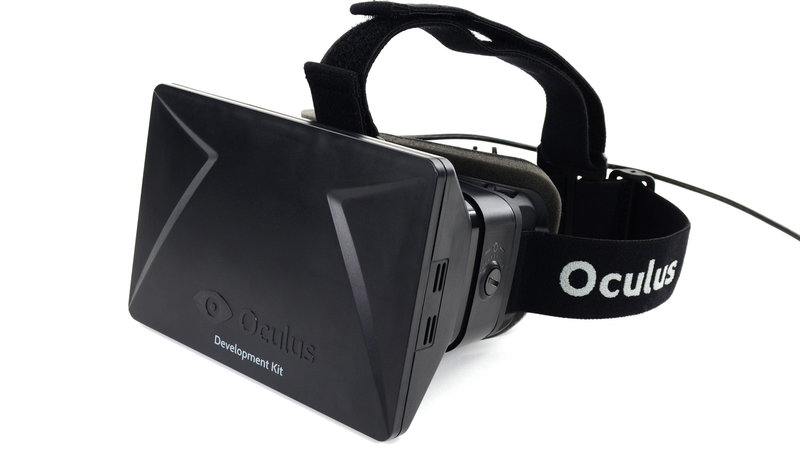
\includegraphics[width=8cm]{oc}
\caption{Oculus Rift}
\label{fig:obrazek k}
\end{figure}

\subsection{Star Citizen}
\label{sec:sc}

Kolejnym przykładem wielkiego sukcesu jest Star Citizen\index{Star Citizen}, gra komputerowa (jeszcze nie powstała), która na kickstarterze\index{Kickstarter} zebrała również ok. 2 milionów dolarów (przy minimalnym progu 500,000\$. To jeszcze nie wszystko, aktualnie studio tworzące grę prowadzi zbiórkę na swojej oficjalnej stronie internetowej i udało im się w ramach tego zebrać okrągłe \textbf{66 milionów dolarów} i ciągle ta kwota rośnie.

Fundusze zgromadzone przez twórców na przestrzeni III i IV kwartału 2013 roku i roku 2014 na podstawie Stretch Goal'i\footnote{Stretch Goal\index{Stretch Goal} - określona suma pieniędzy, po osiągnięciu, której projekt jest rozbudowywany o określone wcześniej ulepszenia.}:

\begin{displaymath}
\left[\begin{array}{cccccc}I poł. 2012&II poł. 2012&I poł. 2013&II poł. 2013&I poł. 2014&II poł.2014\\45,000\$&3,100,000\$&7,500,000\$&11,500,000\$&39,000,000\$&51,500,000\$\\100,000\$&3,500,000\$&8,000,000\$&15,500,000\$&42,000,000\$&59,500,000\$\\500,000\$&5,000,000\$&9,500,000\$&25,000,000\$&44,000,000\$&62,500,000\$\\2,000,000\$&6,000,000\$&10,500,000\$&35,000,000\$&47,000,000\$&66,000,000\$\end{array}\right]
\end{displaymath}

\begin{figure}[ht]
\centering

\includegraphics[width=8cm]{sc}
\caption{Logo Star Citizena}
\label{fig:obrazek k}
\end{figure}

\subsection{Secret Service}
\label{sec:ss}

Ostatni przykład pochodzi z serwisu Polak Potrafi\index{Polak Potrafi} i miał na celu przywrócić na rynek dawny magazyn o grach o nazwie Secret Service\index{Secret Service}. Aktualnie, jest to największy pod względem zebranych środków projekt w Polsce (zebrał 284110 zł). Niestety, wiążą się z nim pewne kontrowersje, co negatywnie odbija się na wizerunku całej inicjatywie crowdfundinu\index{crowdfunding}, otóż pomimio zapewnień autorów projektu, stracili oni prawa do nazwy magazynu i po wydaniu całych dwóch numerów, magazyn nie pokaże się ponownie pod nazwą Secret Service. Wielu z fundatorów czuje się oszukanych i w związku z tym żąda zwrotu pieniędzy zarówno od twórców magazynu jak i od serwisu polakpotrafi.pl. Nie wiadomo jaki finał będzie miała ta sprawa, jednak na pewno nie zrobi dobrej reklamy serwisowi, jak i całej akcji.


\begin{figure}[ht]
\centering

\includegraphics[width=8cm]{ss}
\caption{Logo magazynu}
\label{fig:obrazek k}
\end{figure}

\section{Kontrowersje}

Zwolennicy modelu crowdfoundingu\index{crowdfunding} przekonują, że może on stanowić nie tylko alternatywne źródło finansowania inicjatyw społecznych czy artystycznych, ale też nowych przedsiębiorstw. Z drugiej jednak strony - chodzi o bezpieczeństwo. Projekty, które uzyskały wsparcie internautów, czyli zebrały lub przekroczyły wymaganą kwotę i weszły do produkcji lub sprzedaży, nie zawsze spełniają oczekiwania. Gdy prace się przedłużają, a końcowy produkt odbiega od założeń - tak było z konsolą Ouya\index{Ouya} - to jednak nie najgorszy scenariusz. Gorzej, gdy pomysłodawca projektu po zainkasowaniu wpłaty, nie realizuje obietnic, jak na przykład Tim Shafer. Twórca zebrał kwotę wymaganą, by rozpocząć produkcję nowej gry - ponad 3 miliony dolarów - a po chwili ogłosił po prostu, że jednak potrzebuje więcej.
Jeśli wspierający nie otrzyma swoich „nagród”, a jego pieniądze przepadną, pozostaje mu sąd. Ze względu na nie najwyższe utracone kwoty, jest to jednak rozwiązanie stosowane niezwykle rzadko.

\begin{figure}[!ht]
	\centering
		\includegraphics[width=0.40\textwidth]{rys.pdf}
	\caption{Grafika promocyjna kickstartera}
	\label{fig:rys}
\end{figure}

\newpage

\bibliographystyle{plain}
\begin{thebibliography}{99}

\bibitem{p} Roberts: Roberts Space Industries : www.robertssindrustries.com

\bibitem{a} K. Król: Crowdfunding w Polsce 

\bibitem{t} R. Stanisławski : Oculus Rift czyli klucz do bram wirtualnej rzeczywistości

\bibitem{f} Ł. Wiśniewski : Secret Service to teraz PIXEL. Legenda powróciła na krótko.

\bibitem{q} K. Hildebrand : Co się dzieje z pieniędzmi, jakie przekazujemy twórcom w serwisie Kickstarter?

\end{thebibliography}

\printindex

\end{document}
